\documentclass[a4paper,12pt]{article} 
\usepackage[T2A]{fontenc} %кодировка  
\usepackage[utf8]{inputenc} %Кодировка исходного текста  
\usepackage[english,russian]{babel} %локализация и переносы  
\usepackage[utf8]{inputenc} 
\usepackage[russian]{babel} 
\usepackage{indentfirst} 
\usepackage{float} 
\usepackage{geometry} 
\usepackage[warn]{mathtext} 
\usepackage[english,russian]{babel} 
\usepackage{gensymb} %% Чтоб градусы работали 
\usepackage{amsmath}
\geometry{a4paper,total={170mm,257mm},left=20mm,top=20mm,right=30mm} 
\usepackage{amsmath,amsfonts,amssymb,amsthm,mathtools} %Математика 

 

\title{\textbf{Лабораторная работа №1}\\ Исследование статической системы стабилизации высоты в тангажном варианте} 
\author{Пащенко А.Е.\\Зарубин Р.А.\\Вариант 3} 
\date{} 

\begin{document} 

\maketitle %генерирует титульный лист, который мы задали сверху 
\textbf{Цуль работы:} Исследование методов математического моделирования системы стабилизации высоты на персональном компьюторе.
\section{Теоретический минимум}
Стабилизация высоты полёта может быть достигнута как воздействием на руль высоты, так и посредством изменением тяги. Будем рассматривать наиболее распространённый случай, 
когда скорость полёта постоянна, а высота стабилизируется рулём высоты.\\
В общем видет при постоянной скорости полёта структурная схема высоты показана 
на рис. \ref{fig:1}

\begin{figure}[H]
    \center{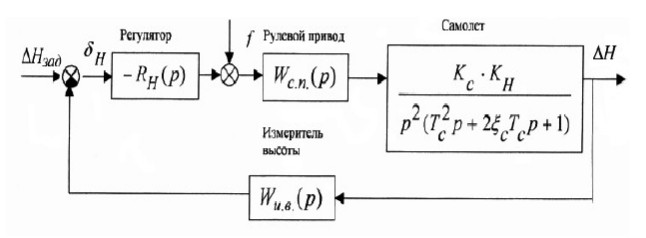
\includegraphics[width=\linewidth]{img/1.jpg}}
    \caption{Структурная схема системы стабилизации высоты}
    \label{fig:1}
\end{figure}
 
Устойчивость такого контура может быть обеспечина двумя путями: \\ 

1) введением внутренней стабилизирующей обратной связи по сигналу угла тангажа 
$\vartheta$, т.е. введением автопилота угла тангажа;\\

2) введением в закон управления $R_{H}(p)$ сигнал первой производной отклонения высоты для случая, если сервопривод имеет жёсткую обратную связь,
и ссумы сигналов первой и всторой производных от сигнала отклонения высоты для случая, 
когдасервопривод имеет скоростную или изодромную обратную связь.\\

На рис. \ref{fig:2} приведена структурная схема системы стабилизации высоты, содержащей автопилот угла тангажа.

\begin{figure}[H]
    \center{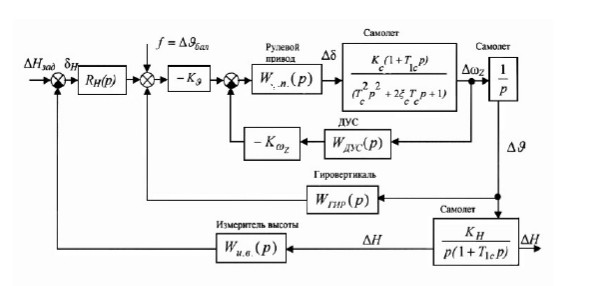
\includegraphics[width=\linewidth]{img/2.jpg}}
    \caption{Структурная схема системы стабилизации высоты}
    \label{fig:2}
\end{figure}

Основным приемуществом такой системы чвляется то, что устойчивость траекторного контура обеспечивается 
регулятором $R_H(p)=i_H$ за счёт сигнала угла тангажа, снимаемого с надёжного датчика -- гировертикали, практически лишённого запаздывания.
Система содержащая регулятор $R_H(p)=i_H$, называется статической системой т.к. этот регулятор не обеспечивает астатизм регулярования в отношении других возмущений. 


\begin{equation}
    \begin{cases}
        \dot{\Delta\alpha}=\Delta\omega_z-\bar{Y}^\alpha_a\Delta\alpha\\
        \dot{\Delta\omega_z} = \bar{M}^\alpha_z\Delta\alpha+\bar{M}^{\omega_z}_z\Delta\omega_z+\bar{M}^{\delta_B}_z\Delta\delta_B\\
        \dot{\Delta\vartheta} = \Delta\omega_z\\
        \dot{\Delta V_y}=V_0\bar{Y}^\alpha_a\Delta\alpha\\
        \dot{\Delta H}=\Delta V_y\\
        \dot{\Delta n_y}=n^\alpha_y\Delta\alpha
    \end{cases}
    \label{eq:СДУ}
\end{equation}

Где система (\ref{eq:СДУ}) -- это система дифференциальных уравнений, используемая для маделирования
движения самолёта в короткопериодическом движении. 

\begin{equation}
    \begin{cases}
        \Delta\delta_B=K_{\omega_z}\Delta\omega_z+K_{\vartheta}(\Delta\vartheta-\Delta\vartheta_{зад}+f)\\
        \Delta\vartheta_{зад} = i_H(\Delta H_{зад}-\Delta H)+i_p\int_{0}^{t}(\Delta H_{зад}-\Delta H)dt
    \end{cases}
    \label{eq:заданные значения}
\end{equation}
 
\section{Выполнение работы}
    \subsection{Исходные данные}

    \begin{table}[H]
        \centering
        \caption{Исходные данные}
        \label{tab:Исходные данные 1}
        \begin{tabular}{|c|c|}
        \hline
            $m_0$ & 25000 кг  \\ \hline
            $S$ & 50 м$^2$ \\ \hline
            $b_a$ & 5м  \\ \hline
            $J_z$ & 50000 кг м$^2$ \\ \hline
            $H$ & 1000 м  \\ \hline
            $M$ & 0,5  \\ \hline
        \end{tabular}
    \end{table}
                                
    \begin{table}[H]
        \centering
        \caption{Исходные данные}
        \label{tab:Исходные данные 2}
        \begin{tabular}{|c|c|}
            \hline
            $\bar{Y}_a^\alpha=a_{11},$ $1/c$ &  0.642  \\ \hline
            $\bar{M}_z^{\alpha}=a_{21}$, $1/c^2$ &   5.65 \\ \hline
            $\bar{M}_z^{\omega_z}=a_{22}$,$1/c$ &  0.468 \\ \hline
            $\bar{M}^{\delta_B}_z=b_2$ & 4.5  \\ \hline
            $V_0=a_{46}$,м$/c$ & 168 \\ \hline
            $n_y^\alpha=a_{51}$ &  11.0  \\ \hline
            $K_{\omega_z}, c$ & 0.4 \\ \hline
            $K_\vartheta$  & 0.5, 1, 2  \\ \hline
            $i_H$ рад/м & 0.000875 0.00175 0.002625 \\ \hline
            $i_p$ рад/м & 0.0000875 0.000175 0.0002625 \\ \hline
            $\hat{t}_{cp},c$ & 8 \\ \hline
            $\hat{\sigma}_{\Delta H}, \%$ & 30 \\ \hline
            $\hat{n}_{y_{max}},c$ & 1.2 \\ \hline
            $\hat{H}_{cm},$ м & 20 \\ \hline
            \end{tabular}
    \end{table}

    \subsection{Ход работы}
    
    \begin{enumerate}
    \item На персональном компьютере установить задачу 1, после чего в цикле для
    каждой   пары   коэффициентов  заданных   в  табл.   1,
    определяются:\\
    а)	при отработке управляющего воздействия  = 100м:
        \begin{itemize}
            \item время срабатывания   
            \item максимальное значение высоты  
            \item максимальное значение перегрузки.
        \end{itemize}
    б)	при отработке постоянного возмущения $f=$ -0.035 рад:
        \begin{itemize}
            \item статическую ошибку регулирования .
        \end{itemize}
    
    Результаты расчетов оформить в виде таблица \ref{tab:Результаты расчётов}.

    %Посчитаные данные
    \begin{table}[H]
        \caption{\label{tab:bolts} Нестандартные болты для левой резьбы.}
            \begin{center}
                \begin{tabular}{|c|c|c|}
                \hline
                & \multicolumn{2}{c|}{Диаметр} \\
                \cline{2-3}
                \raisebox{1.5ex}[0cm][0cm]{Нестандартные болты}
                & Норма & Разброс \\
                \hline
                Размеры & 10 мм & 1 мм \\
                \hline
                \end{tabular}
            \end{center}
        \end{table}

    \item Построить по данным табл. \ref{tab:Результаты расчётов} графики следующих зависимостей:
    $$t_{cp}=f_1(K_{\vartheta},i_H);\sigma_{\Delta H}=f_2(K_{\vartheta},i_H)$$
    $$\Delta n_{y_{max}}=f_3(K_{\vartheta},i_H);\Delta H_{cm}=f_4(K_{\vartheta},i_H)$$
    Нанести   на   графики   прямые   линии,   соответствующие   максимально допустимым величинам показателей качества переходных процессов  $t_{cp}$. 

    $\hat{\sigma}_{\Delta H}$;$\Delta n_{y_{max}}$;$\Delta \hat{H}_{cm}$(смотри табл. \ref{tab:Исходные данные 2})
    
    \begin{figure}[H]     % Графики к пункту 2
        \center{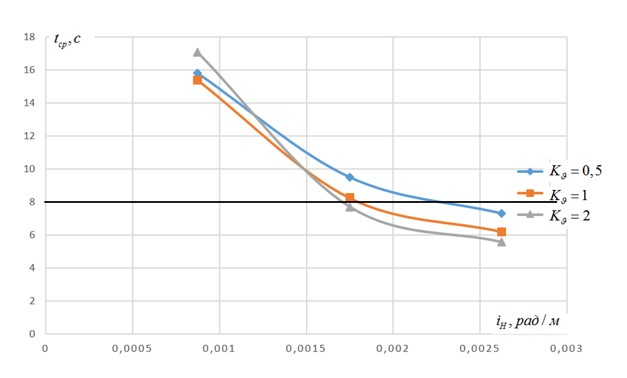
\includegraphics[width=\linewidth]{img/3.jpg}}
        \caption{Время срабатывания $t_{cp}$}
        \label{fig:Время срабатывания}
    \end{figure}
    
    \begin{figure}[H]
        \center{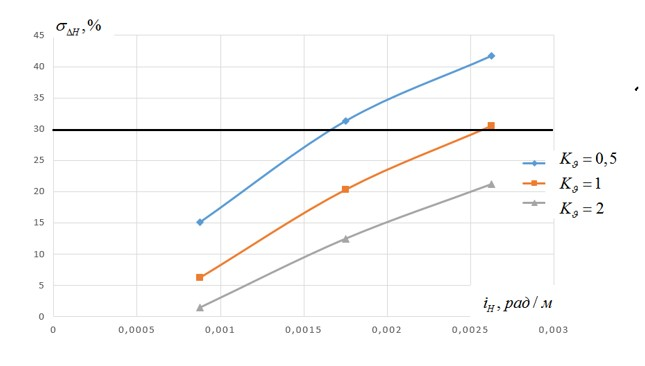
\includegraphics[width=\linewidth]{img/4.jpg}}
        \caption{Относительное перерегулирование $\sigma_{\Delta H}$}
        \label{fig:Относительное перерегулирование}
    \end{figure}
    
    \begin{figure}[H]
        \center{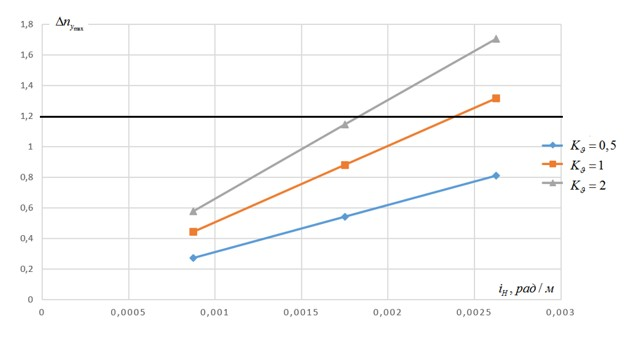
\includegraphics[width=\linewidth]{img/5.jpg}}
        \caption{Максимальное значение нормальной перегрузки $\Delta n_{y_{max}}$}
        \label{fig:Максимальное значение нормальной перегрузки}
    \end{figure}
    
    \begin{figure}[H]
        \center{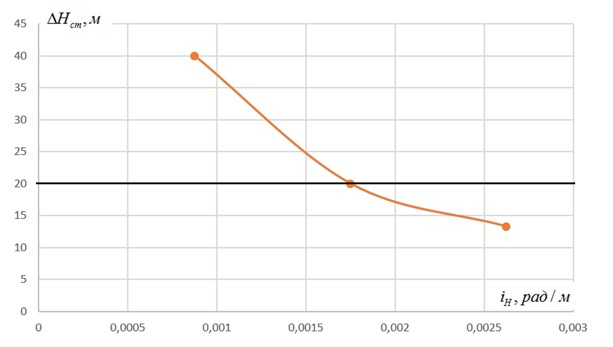
\includegraphics[width=\linewidth]{img/6.jpg}}
        \caption{Статистическая ошибка по высоте $\Delta H_{cm}$}
        \label{fig:Статистическая ошибка по высоте}
    \end{figure}


    \item Построить, используя зависимости п. 2, допустимую область изменения коэффициентов усиления $K_{\vartheta}=f(i_H)$ из условия \\ $t_{cp} \leq \hat{t}_{cp}$; $\sigma_{\Delta H} \leq \hat{\sigma}_{\Delta H_{cp}}$;
    $\Delta n_{y_{max}} \leq \Delta \hat{n}_{y{max}}$; $\Delta H_{cm} \leq \Delta \hat{H}_{cm}$  

    % Графики пункта 3
    \begin{figure}[H]
        \center{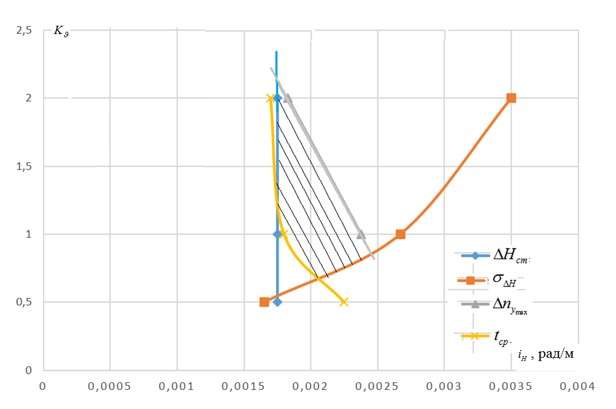
\includegraphics[width=\linewidth]{img/7.jpg}}
        \caption{Область изменения коэффициента усиления}
        \label{fig:Область изменения коэффициента усиления}
    \end{figure}

    \end{enumerate}
    
    \subsection{Переходные процессы}

    \begin{figure}[H]
        \center{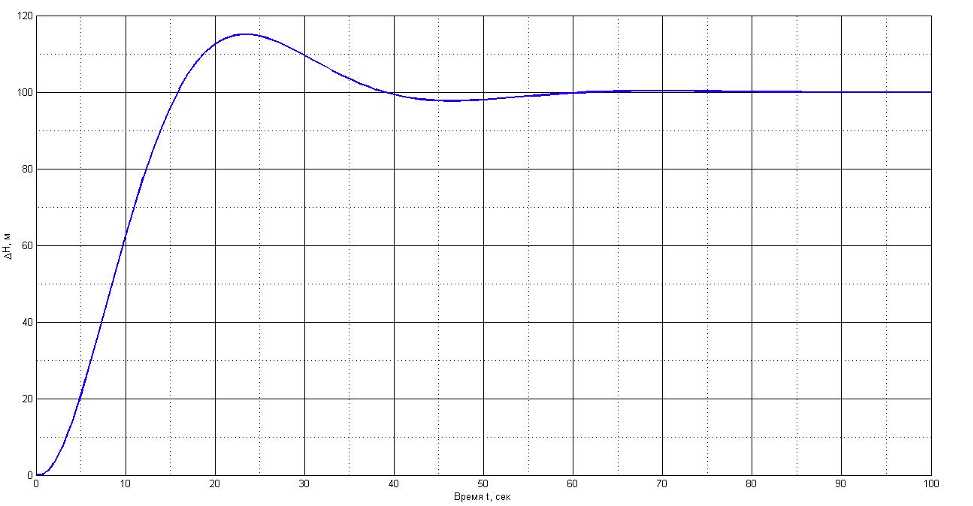
\includegraphics[width=\linewidth]{img/8.png}}
        \caption{График ппереходного процесса при $K_{\vartheta}=0.5, i_H=0,000875$ [рад/м], $f=0$}
        \label{fig:Переходный процесс 1}
    \end{figure}

    \begin{figure}[H]
        \center{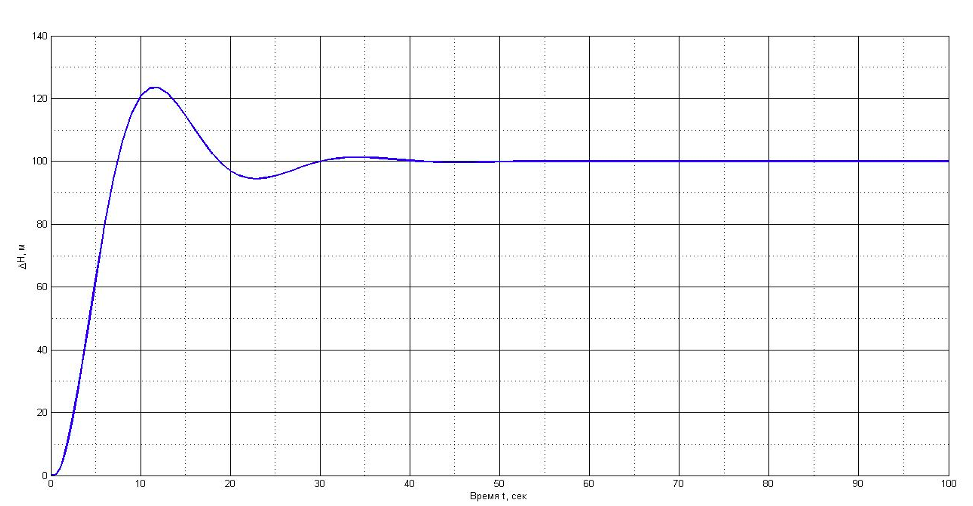
\includegraphics[width=\linewidth]{img/9.png}}
        \caption{График ппереходного процесса при $K_{\vartheta}=1, i_H=0,002$[рад/м], $f=0$}
        \label{fig:Переходный процесс 2}
    \end{figure}

    \subsection{Выводы}
    \begin{enumerate}
        \item Статическая ошибка, возникающая при наличии возмущений, уменьшается с увеличением коэффициентов стабилизации.
        \item При увеличении $K_{\vartheta}$  и $i_H$, рад/м время срабатывания системы уменьшается.
        \item При увеличении коэффициентов $K_{\vartheta}$  и $i_H$ $\Delta n_{y_{max}}$ возрастает. 
        \item Относительное перерегулирование при увеличении коэффициента $K_{\vartheta}$ уменьшается, а при увеличении $i_H$ увеличивается.
    \end{enumerate}



\end{document} 
